\chapter{Les profils UML}
%OMG Unified Modeling LanguageTM (OMG UML),Superstructure
\label{chap.profils-UML}
\section{Le langage de modélisation UML}

Le \glsfirst{uml} est un langage de modélisation standardisé permettant de créer des mod\`eles, typiquement sous forme de diagrammes.
Ces diagrammes permettent de visualiser, spécifier, construire et documenter des logiciels, des systèmes et des processus d'affaire.
UML utilise des diverses notations,  surtout graphiques, pour exprimer le design et l'architecture de projets logiciels.
Les spécifications du standard UML sont en ligne sur le site de l'OMG (\emph{Object Management Group})~\cite{OMG_UML}.

\gt{Comme indiqu\'e pr\'ec\'emment, sauf certaines exceptions, on
n'utilise pas trop le positionnement [H], i.e., on laisse flotter, on
laisse \LaTeX\ d\'ecider o\`u mettre la figure. Par contre, on met les
figures ou tableaux *avant* la r\'ef\'erence.}

\begin{figure}
    \centering
    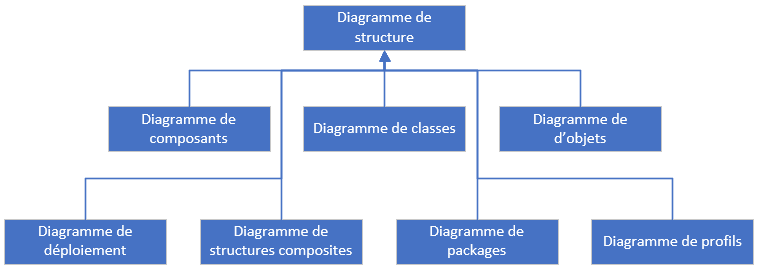
\includegraphics[width=12cm]{10_img/chap4/structure.PNG}
    \caption{Les principaux types de diagrammes de structure d'UML~\cite{OMG_UML}.}
    \label{fig.uml_struc}
\end{figure}

\begin{figure}
    \centering
    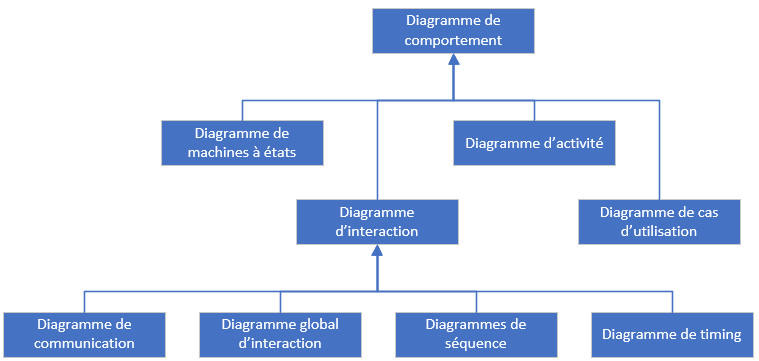
\includegraphics[width=12cm]{10_img/chap4/comportement.PNG}
    \caption{Les principaux types de diagrammes de comportement d'UML~\cite{OMG_UML}.}
    \label{fig.uml_comp}
\end{figure}


\gt{Il vaut mieux utiliser une forme <<active>> --- <<La figure
pr\'esente>> --- qu'une forme passive --- <<Dans la figure sont
pr\'esent\'es\ldots>>.}

La figure~\ref{fig.uml_struc} présente les principaux types de diagrammes de structure proposés par UML,
alors que la figure~\ref{fig.uml_comp} présente les principaux types de diagrammes de comportement.

UML \'etant langage de modélisation largement connu et bien documenté dans le domaine du g\'enie logiciel,
nous nous concentrerons dans le pr\'esent chapitre plus particulièrement à définir les notions nécessaires à la compréhension des mécanismes et des éléments composant les profils UML.



\section{La notion de profil en UML}

\gt{UML pr\'esente diverses notions, qui peuvent \^etre
repr\'esent\'ees de fa\c{c}on graphique ou textuelle.  Donc, en soit,
aucun item UML n'est un diagramme.  Le diagramme est une des
repr\'esentations possibles d'une notion.}


Un profil UML est une forme de m\'ecanisme d'extension, qui
permet d'étendre les mécanismes d'UML afin d'adapter les mod\`eles et leur contenu à un domaine particulier (par ex.,  domaines d'activité spécifique) ou \`a une plateforme particulière (par ex.,  .NET, J2EE).

Les extensions qu'un profil d\'efinit permettent d'ajouter des caractéristiques aux éléments standards d'UML.
Elles ne permettent pas de retirer des caractéristiques des éléments, et ce pour ne pas aller à l'encontre de la sémantique standard d'UML.
Un profil se compose  de stéréotypes, de valeurs \'etiquet\'ees (\emph{tagged values}) et de contraintes qui s'appliquent aux éléments de modèles UML tels que les classes, les attributs, les opérations et les activités.

\subsection{Un exemple d'application}
Afin de mieux comprendre les éléments qui composent un profil, nous allons mettre en place un exemple d'application au fur et à mesure de ce chapitre, en y intégrant divers éléments un \`a la fois.

\begin{figure}
    \centering
    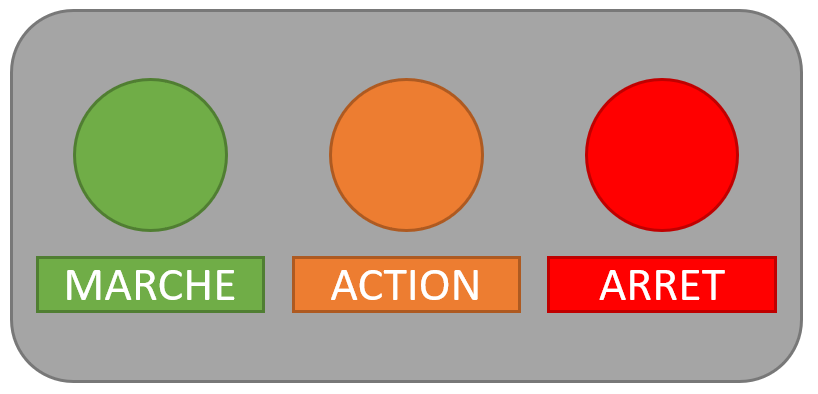
\includegraphics[width=8cm]{10_img/chap4/example.PNG}
    \caption{Le tableau de bord de la machine pour notre exemple de profil UML.}
    \label{fig.uml_ex}
\end{figure}

Prenons un exemple d'un mod\`ele devant représenter un tableau de bord d'une machine composé de trois boutons : \texttt{Marche}, \texttt{Action}, \texttt{Arrêt}.
Chaque bouton a un état <<actif>> ou <<inactif>>, et
chacun a une action qui lui est propre sur la machine contr\^ol\'ee par ces boutons : \texttt{Marche} = démarre la machine; \texttt{Action} = effectue l'action de la machine; \texttt{Arrêt} = termine l'ex\'ecution de la machine.
%
La figure~\ref{fig.uml_ex} illustre le tableau de bord de cette machine.

%\newpage \GT{A EVITER, sauf a la toute fin, quand on veut fignoler la mise en page!}

\section{Les stéréotypes}
\label{sect.uml.ster}
Les stéréotypes permettent d'appliquer des extensions aux métaclasses UML.
Plus pr\'ecis\'ement, il permettent d'ajouter des termes spécifiques de vocabulaire à un mod\`ele.
Un stéréotype s'applique à un mod\`ele UML, permettant ainsi de le rendre spécifique à un domaine en y appliquant des propriétés spécifiques.

\subsection{Un exemple d'application}

\begin{figure}
    \begin{center}
    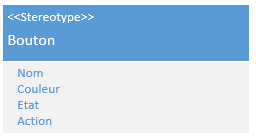
\includegraphics[width=5cm]{10_img/chap4/button.PNG}
    \caption{Un st\'er\'eotype <<\texttt{Bouton}>> permettant de sp\'ecifier les points communs aux diff\'erents boutons.}
    \label{fig.uml_but_definition}
    \end{center}
\end{figure}


\gt{Dans la figure \ref{fig.uml_but_definition}, tu dois \^etre plus explicite
quant au fait que cela \'etend une classe.
%
Donc, ta boite/classe Bouton doit \^etre une sous-classe d'une boite contenant "<<metaclass>> Class".
%
Voir d\'ebut de la page \url{https://www.uml-diagrams.org/stereotype.html}.}

\gt{Tu devrais utiliser ce stereotype pour d\'efinir au moins un des
boutons, par ex.: "<<bouton>> Marche". Cf. partie <<Stereotype
Application>> de
\url{https://www.uml-diagrams.org/stereotype.html}. Pr\'ef\'erablement
dans une autre figure, possiblement dans la section Tagged values.
Parce que l\`a, tu introduis le stereotype Bouton, mais ensuite tu
utilise celui de Machine, qui n'est pas d\'efini!}



Dans notre exemple, nous avons plusieurs éléments : un tableau de bord, des boutons, des actions que les boutons effectuent.
Un stéréotype, comme celui présent dans la figure~\ref{fig.uml_but_definition}, pourrait être d\'efini afin de sp\'ecifier les caractéristiques communes des boutons.
%
Une fois d\'efini, ce st\'er\'eotype pourra alors \^etre utilis\'e pour
d\'efinir diff\'erentes instances de \texttt{Bouton} --- voir ci-bas (Figure~\ref{fig.uml_marche}).


%\newpage

\section{Les valeurs \'etiquet\'ees}

Les valeurs \'etiquet\'ees (\emph{tagged values}) permettent d'ajouter \`a un \'el\'ement des propriétés qui lui sont spécifiques.
Plus pr\'ecis\'ement, ce m\'ecanisme permet d'ajouter de l'information spécifique aux éléments \`a l'aide de paires clé/valeur.
Les attributs présents dans un stereotype seront affichés visuellement dans une classe faisant usage du stéréotype.
Ces couples clé-valeur se trouveront entre crochet sous le nom de la classe comme dans la Figure~\ref{fig.uml_marche}.

\gt{Je ne comprends pas la derni\`ere phrase!?}

\subsection{Un exemple d'application}

\begin{figure}
    \begin{center}
    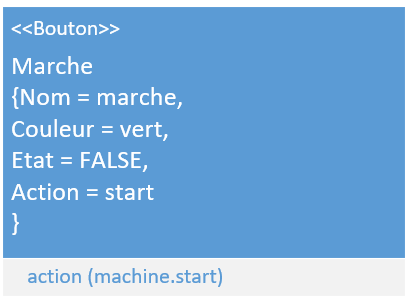
\includegraphics[width=5cm]{10_img/chap4/start.PNG}
    \caption{Des valeurs \'etiquet\'ees permettant de spécifier le bouton \texttt{Marche}}
    \label{fig.uml_marche}
    \end{center}
\end{figure}

Dans notre exemple, nous pouvons supposer que la machine est un modèle spécifique et donc que le diagramme ne s'applique qu'à ce modèle précis (par ex., Modèle 1.2.3).
Nous trouverons donc dans notre diagramme UML la notation de la figure~\ref{fig.uml_marche}.

\gt{Je crois, comme indiqu\'e plus haut, qu'une utilisation de Bouton serait pr\'ef\'erable.}

%\newpage

\section{Les contraintes}
Les contraintes sont des propriétés spécifiques, qui permettent de sp\'ecifier des conditions additionnelles sur un modèle.
Ces conditions peuvent être appliquées à une ou plusieurs classes, à un ou plusieurs attributs, à une ou plusieurs relations entre classes.
Une contrainte est représent\'ee, dans un modèle, sous la forme d'une note indiquant une phrase qui exprimant la contrainte entre crochets ou encore, de fa\c{c}on plus formelle, sous la forme d'une contrainte OCL~\cite{OCL}.

\subsection{Un exemple d'application}

\begin{figure}
    \begin{center}
    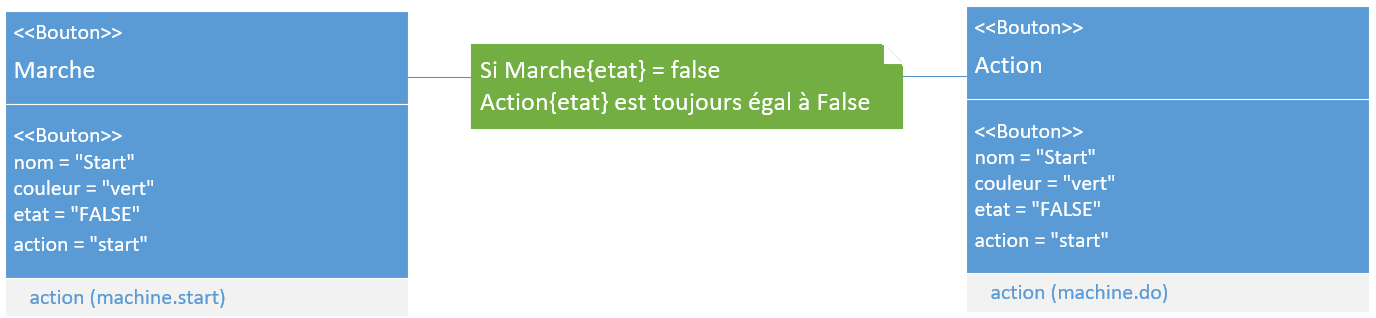
\includegraphics[width=12cm]{10_img/chap4/constraint.PNG}
    \caption{Des contrainte permettant de sp\'ecifier des conditions sur des \'el\'ements d'un modèle.}
    \label{fig.uml_con}
    \end{center}
\end{figure}

Dans notre exemple, nous pouvons supposer la contrainte suivante : l'action de la machine ne peut pas être effectuée si la machine est à l'arrêt.
Nous pourrons alors sp\'ecifier, dans notre diagramme UML, la contrainte présent\'ee dans la figure~\ref{fig.uml_con}.

%\newpage

\section{Les ic\^ones}
Lorsqu'un modèle devient important en taille il peut devenir difficile de s'y retrouver parmi les nombreux st\'er\'eotypes.
Cependant, l'association d'ic\^ones aux st\'er\'eotypes peut être une solution int\'eressante à mettre en place dans le cas d'un profil dans un domaine d'activité spécifique.
Une représentation graphique simple --- une ic\^one --- peut ainsi être attribuée à un type d'élément spécifique du modèle.

\subsection{Un exemple d'application}


\begin{figure}
    \begin{center}
    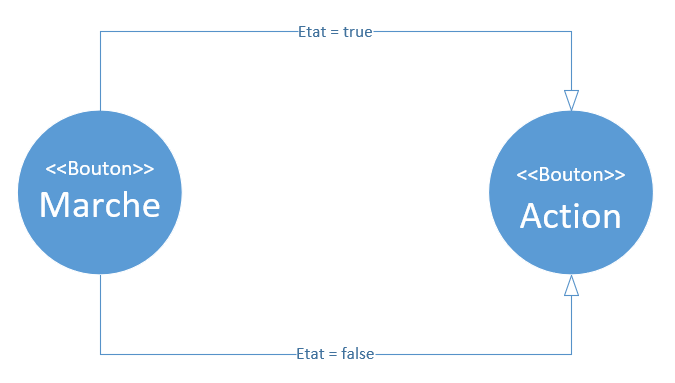
\includegraphics[width=12cm]{10_img/chap4/img.PNG}
    \caption{Une ic\^one spécifique associ\'ee aux boutons.}
    \label{fig.uml_img}
    \end{center}
\end{figure}

Dans notre environnement, nous avons une machine composée de trois boutons.
Nous pouvons, par exemple, décider d'attribuer une ic\^one spécifique aux boutons afin de les différencier des autres éléments, tel qu'illustr\'e dans la figure~\ref{fig.uml_img}.



%\newpage

\section{L'utilisation d'un profil UML pour la conception de jeux vidéos}


UML est un langage de modélisation permettant de représenter divers types de systèmes et permettant de les documenter de manière rigoureuse en apportant les caractéristiques suivantes :

\begin{itemize}
    \item UML est un langage formel et normalisé;
    \item UML est manipulable avec de nombreux outils déjà approuvés;
    \item UML est un support de communication performant;
    \item UML est un langage qui permet le \emph{versionning} et la conservation de l'information de manière efficace.
\end{itemize}

\gt{Ci-haut: Pas certain que j'aime la comparaison avec les mind maps.
Dans mon esprit, un mind map a un r\^ole tout \`a fait diff\'erent ---
plus exploratoire, parce que plus libre, avec moins de
contraintes. Donc, je crois que tes items pourraient rester, mais sans
insister sp\'ecifiquement que c'est par rapport aux mind maps.}



Cependant, UML est un langage de modélisation tellement étendu qu'il permet de tout faire, ce qui rend le langage difficile à appréhender.
De plus, UML est prévu à l'origine afin de représenter des systèmes logiciels, donc le vocabulaire utilisé est spécifique à la programmation informatique.


Dans les chapitres précédents, nous avons établi une liste de points importants concernant la conception de jeux vidéos.
Nous pensons qu'un profil UML serait un outil int\'eressant pour répondre aux besoins de modélisation d'un GDD.
La mise en place d'un profil UML aurait plusieurs avantages :
\begin{itemize}
    \item Les outils supportant UML sont nombreux et efficaces. Ils sont déjà présents sur le marché et répondent aux besoins de la modélisation UML.

    \item En utilisant un profil il est possible de simplifier la compréhension des différents objets UML à utiliser pour exprimer un concept, ce qui permet de réduire la quantité de connaissances à acquérir pour se servir d'UML dans le cadre de la rédaction d'un GDD.

    \item Les stéréotypes permettent d'intégrer des notions spécifiques au \emph{game design}.

    \item Les valeurs \'etiquet\'ees permettent d'ajouter des propriétés spécifiques aux nouveaux éléments introduits par les st\'er\'eotypes.

    \item Des contraintes peuvent être sp\'ecifi\'ees dans un profil afin d'éviter des erreurs.

    \item Des ic\^ones peuvent être associ\'ees aux éléments du modèle pour faciliter sa compréhension.
\end{itemize}


\gt{Ci-haut: 2e item: je ne comprends l'histoire de <<port\'ee>> des objets!?}

Grâce aux ajustements et extensions permis par les profils, UML semble être un langage int\'eressant pour permettre la représentation graphique d'un GDD.
C'est pourquoi dans le Chapitre~\ref{game-genesis.sect} nous proposons un profil UML permettant la description des éléments d'un GDD.
